\documentclass[]{book}
\usepackage{lmodern}
\usepackage{amssymb,amsmath}
\usepackage{ifxetex,ifluatex}
\usepackage{fixltx2e} % provides \textsubscript
\ifnum 0\ifxetex 1\fi\ifluatex 1\fi=0 % if pdftex
  \usepackage[T1]{fontenc}
  \usepackage[utf8]{inputenc}
\else % if luatex or xelatex
  \ifxetex
    \usepackage{mathspec}
  \else
    \usepackage{fontspec}
  \fi
  \defaultfontfeatures{Ligatures=TeX,Scale=MatchLowercase}
\fi
% use upquote if available, for straight quotes in verbatim environments
\IfFileExists{upquote.sty}{\usepackage{upquote}}{}
% use microtype if available
\IfFileExists{microtype.sty}{%
\usepackage{microtype}
\UseMicrotypeSet[protrusion]{basicmath} % disable protrusion for tt fonts
}{}
\usepackage[margin=1in]{geometry}
\usepackage{hyperref}
\hypersetup{unicode=true,
            pdftitle={Data Mining for Student Success and Perseverance},
            pdfauthor={Sameer Bhatnagar; Jonathan Guillemette; Micheal Dugdale; Sahir Bhatnagar; Nathaniel Lasry},
            pdfborder={0 0 0},
            breaklinks=true}
\urlstyle{same}  % don't use monospace font for urls
\usepackage{natbib}
\bibliographystyle{apalike}
\usepackage{longtable,booktabs}
\usepackage{graphicx,grffile}
\makeatletter
\def\maxwidth{\ifdim\Gin@nat@width>\linewidth\linewidth\else\Gin@nat@width\fi}
\def\maxheight{\ifdim\Gin@nat@height>\textheight\textheight\else\Gin@nat@height\fi}
\makeatother
% Scale images if necessary, so that they will not overflow the page
% margins by default, and it is still possible to overwrite the defaults
% using explicit options in \includegraphics[width, height, ...]{}
\setkeys{Gin}{width=\maxwidth,height=\maxheight,keepaspectratio}
\IfFileExists{parskip.sty}{%
\usepackage{parskip}
}{% else
\setlength{\parindent}{0pt}
\setlength{\parskip}{6pt plus 2pt minus 1pt}
}
\setlength{\emergencystretch}{3em}  % prevent overfull lines
\providecommand{\tightlist}{%
  \setlength{\itemsep}{0pt}\setlength{\parskip}{0pt}}
\setcounter{secnumdepth}{5}
% Redefines (sub)paragraphs to behave more like sections
\ifx\paragraph\undefined\else
\let\oldparagraph\paragraph
\renewcommand{\paragraph}[1]{\oldparagraph{#1}\mbox{}}
\fi
\ifx\subparagraph\undefined\else
\let\oldsubparagraph\subparagraph
\renewcommand{\subparagraph}[1]{\oldsubparagraph{#1}\mbox{}}
\fi

%%% Use protect on footnotes to avoid problems with footnotes in titles
\let\rmarkdownfootnote\footnote%
\def\footnote{\protect\rmarkdownfootnote}

%%% Change title format to be more compact
\usepackage{titling}

% Create subtitle command for use in maketitle
\newcommand{\subtitle}[1]{
  \posttitle{
    \begin{center}\large#1\end{center}
    }
}

\setlength{\droptitle}{-2em}
  \title{Data Mining for Student Success and Perseverance}
  \pretitle{\vspace{\droptitle}\centering\huge}
  \posttitle{\par}
  \author{Sameer Bhatnagar \\ Jonathan Guillemette \\ Micheal Dugdale \\ Sahir Bhatnagar \\ Nathaniel Lasry}
  \preauthor{\centering\large\emph}
  \postauthor{\par}
  \predate{\centering\large\emph}
  \postdate{\par}
  \date{2017-05-26}

\usepackage{booktabs}
\usepackage{amsthm}
\makeatletter
\def\thm@space@setup{%
  \thm@preskip=8pt plus 2pt minus 4pt
  \thm@postskip=\thm@preskip
}
\makeatother

\usepackage{amsthm}
\newtheorem{theorem}{Theorem}[chapter]
\newtheorem{lemma}{Lemma}[chapter]
\theoremstyle{definition}
\newtheorem{definition}{Definition}[chapter]
\newtheorem{corollary}{Corollary}[chapter]
\newtheorem{proposition}{Proposition}[chapter]
\theoremstyle{definition}
\newtheorem{example}{Example}[chapter]
\theoremstyle{remark}
\newtheorem*{remark}{Remark}
\begin{document}
\maketitle

{
\setcounter{tocdepth}{1}
\tableofcontents
}
\chapter{Preface}\label{preface}

This report summarizes the work done by our team on using college
registration records at three diffrenet anglophone CEGEPS in Montreal in
order to find predictors of attrition.

\chapter{Introduction}\label{intro}

\chapter{Literature}\label{literature}

The most important relevant work for this project is
\citep{jorgensen_predicting_2009}.

\chapter{Descriptive Statistics}\label{descriptive-statistics}

Here in we will describe - the data set - the methods by which we label
students at risk - the distributions of at-risk students by -
demographic indicators - registration record indicators

\section{Demographics across the colleges and major
programs}\label{demographics-across-the-colleges-and-major-programs}

\section{Fraction of students who change
colleges}\label{fraction-of-students-who-change-colleges}

\chapter{Methods Centered on Determining Predictive
Factors}\label{methods-centered-on-determining-predictive-factors}

This chapter will be focused on methods which have a sound probabilistic
framework, and allow for inference into the statistical importance of
predictive factors.

\begin{itemize}
\tightlist
\item
  Logistic Regression
\item
  Mixed Effects Models
\end{itemize}

\chapter{Methods centered on predicting at-risk
students}\label{methods-centered-on-predicting-at-risk-students}

This chapter will explore the use of machine learning algorithms whose
primary focus is prediction. This comes at the expense of model
interpretatbility, and this tradeoff will be discussed herein as well.

\begin{itemize}
\tightlist
\item
  Decision Trees and Random Forests
\item
  Neural Networks
\end{itemize}

\section{Example one}\label{example-one}

\section{Example two}\label{example-two}

\chapter{Comparisons}\label{comparisons}

This chapter will compare the effectiveness of the methods developped in
the previous two chapters, and compare them to more basic approaches to
identifying students at-risk.

For example, we know that some CEGEPs have implemented a policy whereby
they identify students as being at risk based on their mid-term
assessments: if the student receives a certain number of ``at-risk'' or
``failing'' results, they are automatically sent an email referring them
to academic support services.

Based on this, we can ask the following research questions : - how
effective is this approach at identifying students who drop-out? - how
does this approach compare to our models from the previous chapters?

We begin with a basic logistic regression with demographic variables,
and as well as the number of each type of results of mid-term
assessment, for students in their last term at the college. With these
predictors, we try to predict if students are about to graduate, or
simply not register again.

\begin{longtable}[]{@{}ccccc@{}}
\toprule
\begin{minipage}[b]{0.30\columnwidth}\centering\strut
~\strut
\end{minipage} & \begin{minipage}[b]{0.13\columnwidth}\centering\strut
Estimate\strut
\end{minipage} & \begin{minipage}[b]{0.16\columnwidth}\centering\strut
Std. Error\strut
\end{minipage} & \begin{minipage}[b]{0.12\columnwidth}\centering\strut
z value\strut
\end{minipage} & \begin{minipage}[b]{0.12\columnwidth}\centering\strut
Pr(\textgreater{}\textbar{}z\textbar{})\strut
\end{minipage}\tabularnewline
\midrule
\endhead
\begin{minipage}[t]{0.30\columnwidth}\centering\strut
\textbf{num\_pass}\strut
\end{minipage} & \begin{minipage}[t]{0.13\columnwidth}\centering\strut
0.5877\strut
\end{minipage} & \begin{minipage}[t]{0.16\columnwidth}\centering\strut
0.02321\strut
\end{minipage} & \begin{minipage}[t]{0.12\columnwidth}\centering\strut
25.32\strut
\end{minipage} & \begin{minipage}[t]{0.12\columnwidth}\centering\strut
1.747e-141\strut
\end{minipage}\tabularnewline
\begin{minipage}[t]{0.30\columnwidth}\centering\strut
\textbf{num\_at\_risk}\strut
\end{minipage} & \begin{minipage}[t]{0.13\columnwidth}\centering\strut
1.455\strut
\end{minipage} & \begin{minipage}[t]{0.16\columnwidth}\centering\strut
0.03664\strut
\end{minipage} & \begin{minipage}[t]{0.12\columnwidth}\centering\strut
39.7\strut
\end{minipage} & \begin{minipage}[t]{0.12\columnwidth}\centering\strut
0\strut
\end{minipage}\tabularnewline
\begin{minipage}[t]{0.30\columnwidth}\centering\strut
\textbf{num\_failing}\strut
\end{minipage} & \begin{minipage}[t]{0.13\columnwidth}\centering\strut
2.193\strut
\end{minipage} & \begin{minipage}[t]{0.16\columnwidth}\centering\strut
0.04653\strut
\end{minipage} & \begin{minipage}[t]{0.12\columnwidth}\centering\strut
47.15\strut
\end{minipage} & \begin{minipage}[t]{0.12\columnwidth}\centering\strut
0\strut
\end{minipage}\tabularnewline
\begin{minipage}[t]{0.30\columnwidth}\centering\strut
\textbf{num\_courses}\strut
\end{minipage} & \begin{minipage}[t]{0.13\columnwidth}\centering\strut
-0.7442\strut
\end{minipage} & \begin{minipage}[t]{0.16\columnwidth}\centering\strut
0.02373\strut
\end{minipage} & \begin{minipage}[t]{0.12\columnwidth}\centering\strut
-31.36\strut
\end{minipage} & \begin{minipage}[t]{0.12\columnwidth}\centering\strut
6.315e-216\strut
\end{minipage}\tabularnewline
\begin{minipage}[t]{0.30\columnwidth}\centering\strut
\textbf{SexeM}\strut
\end{minipage} & \begin{minipage}[t]{0.13\columnwidth}\centering\strut
0.2111\strut
\end{minipage} & \begin{minipage}[t]{0.16\columnwidth}\centering\strut
0.0386\strut
\end{minipage} & \begin{minipage}[t]{0.12\columnwidth}\centering\strut
5.469\strut
\end{minipage} & \begin{minipage}[t]{0.12\columnwidth}\centering\strut
4.537e-08\strut
\end{minipage}\tabularnewline
\begin{minipage}[t]{0.30\columnwidth}\centering\strut
\textbf{birth\_placeQuebec}\strut
\end{minipage} & \begin{minipage}[t]{0.13\columnwidth}\centering\strut
-0.5914\strut
\end{minipage} & \begin{minipage}[t]{0.16\columnwidth}\centering\strut
0.04815\strut
\end{minipage} & \begin{minipage}[t]{0.12\columnwidth}\centering\strut
-12.28\strut
\end{minipage} & \begin{minipage}[t]{0.12\columnwidth}\centering\strut
1.108e-34\strut
\end{minipage}\tabularnewline
\begin{minipage}[t]{0.30\columnwidth}\centering\strut
\textbf{LangueMaternelleAU}\strut
\end{minipage} & \begin{minipage}[t]{0.13\columnwidth}\centering\strut
-0.193\strut
\end{minipage} & \begin{minipage}[t]{0.16\columnwidth}\centering\strut
0.05173\strut
\end{minipage} & \begin{minipage}[t]{0.12\columnwidth}\centering\strut
-3.731\strut
\end{minipage} & \begin{minipage}[t]{0.12\columnwidth}\centering\strut
0.0001907\strut
\end{minipage}\tabularnewline
\begin{minipage}[t]{0.30\columnwidth}\centering\strut
\textbf{LangueMaternelleFR}\strut
\end{minipage} & \begin{minipage}[t]{0.13\columnwidth}\centering\strut
0.3504\strut
\end{minipage} & \begin{minipage}[t]{0.16\columnwidth}\centering\strut
0.04914\strut
\end{minipage} & \begin{minipage}[t]{0.12\columnwidth}\centering\strut
7.13\strut
\end{minipage} & \begin{minipage}[t]{0.12\columnwidth}\centering\strut
1.006e-12\strut
\end{minipage}\tabularnewline
\begin{minipage}[t]{0.30\columnwidth}\centering\strut
\textbf{(Intercept)}\strut
\end{minipage} & \begin{minipage}[t]{0.13\columnwidth}\centering\strut
0.5654\strut
\end{minipage} & \begin{minipage}[t]{0.16\columnwidth}\centering\strut
0.0694\strut
\end{minipage} & \begin{minipage}[t]{0.12\columnwidth}\centering\strut
8.147\strut
\end{minipage} & \begin{minipage}[t]{0.12\columnwidth}\centering\strut
3.741e-16\strut
\end{minipage}\tabularnewline
\bottomrule
\end{longtable}

(Dispersion parameter for binomial family taken to be 1 )

\begin{longtable}[]{@{}cl@{}}
\toprule
\begin{minipage}[t]{0.25\columnwidth}\centering\strut
Null deviance:\strut
\end{minipage} & \begin{minipage}[t]{0.35\columnwidth}\raggedright\strut
24452 on 18370 degrees of freedom\strut
\end{minipage}\tabularnewline
\begin{minipage}[t]{0.25\columnwidth}\centering\strut
Residual deviance:\strut
\end{minipage} & \begin{minipage}[t]{0.35\columnwidth}\raggedright\strut
17188 on 18362 degrees of freedom\strut
\end{minipage}\tabularnewline
\bottomrule
\end{longtable}

\chapter{Continuing Education at
Dawson}\label{continuing-education-at-dawson}

The department of Continuing at Education offers evening courses across
many disciplines throughout the year. The purpose of this report is to
give a broad overview of the demographics and sector-level metrics for
students taking courses within Cont Ed.

\section{Services}\label{services}

Herein, we look at the services offered by the Division of Continuing
Education.

\subsection{Continuing Education's Growth over
Time}\label{continuing-educations-growth-over-time}

How have each of the departments increased their ContEd offerings over
time?

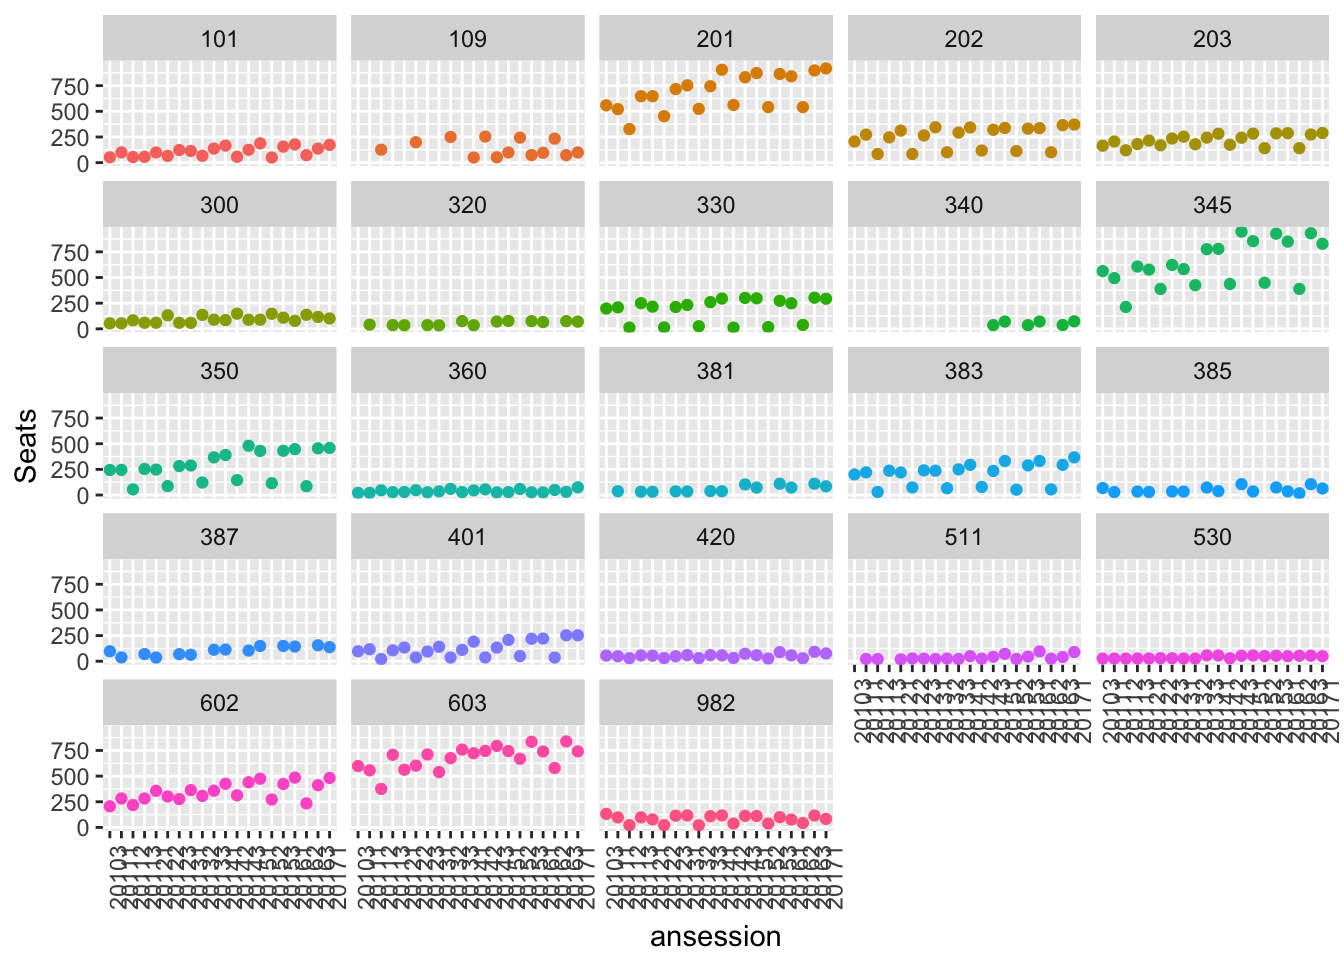
\includegraphics{studentsuccess_final_report_files/figure-latex/dept-level-sizes-over-time-1.pdf}

\subsection{Department Level Seat
Distributions}\label{department-level-seat-distributions}

Which parts of Continuing Education are the most important in 2016?

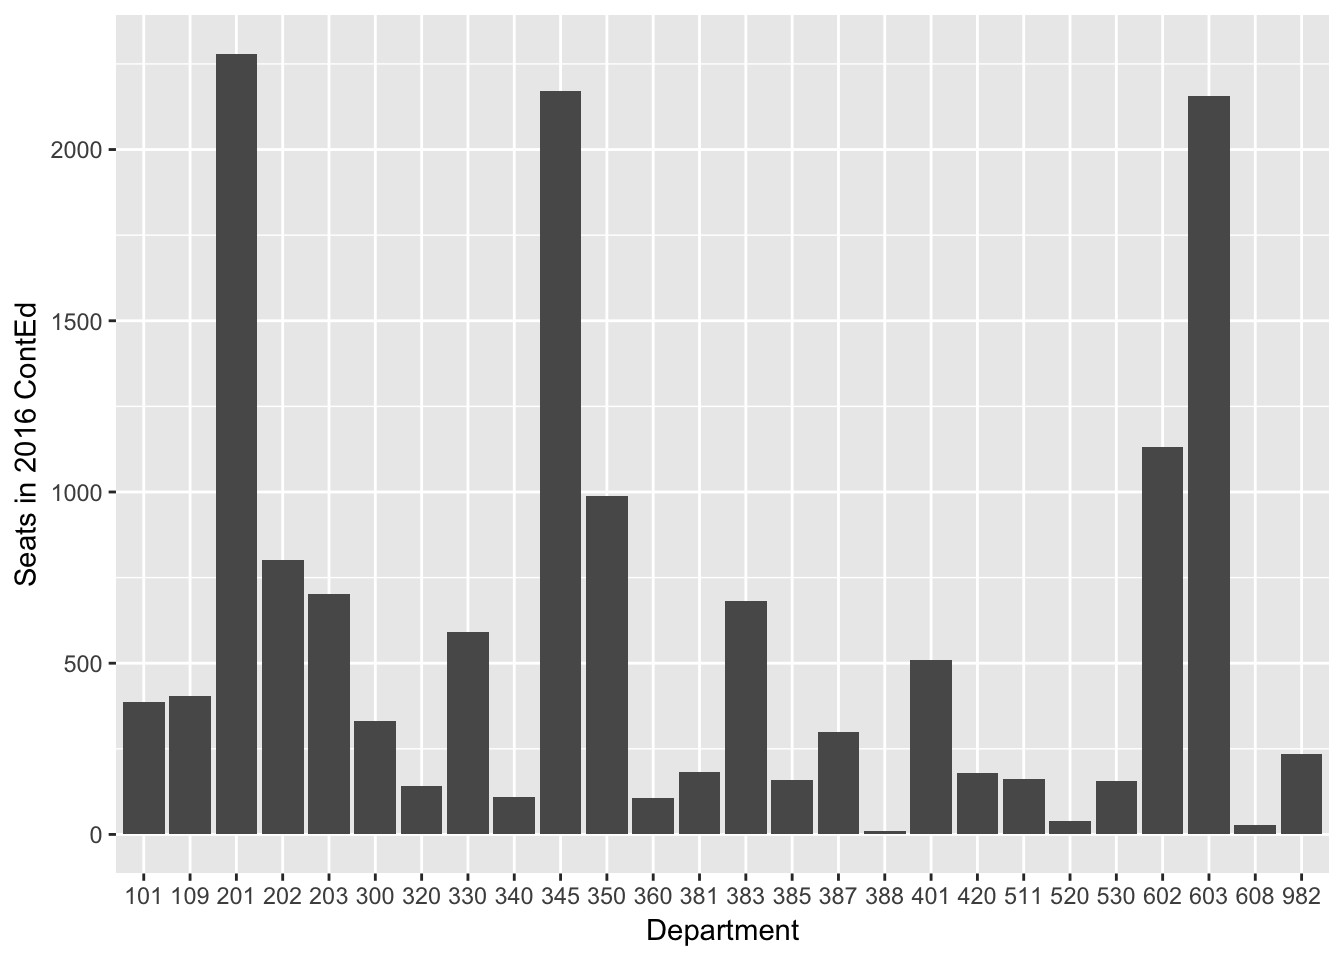
\includegraphics{studentsuccess_final_report_files/figure-latex/dept-level-sizes-2016-1.pdf}

\subsection{Course Level
distributions}\label{course-level-distributions}

If we look at the three most important departments (Math,Humanities and
English) in 2016, how are the seats distrinuted across courses?

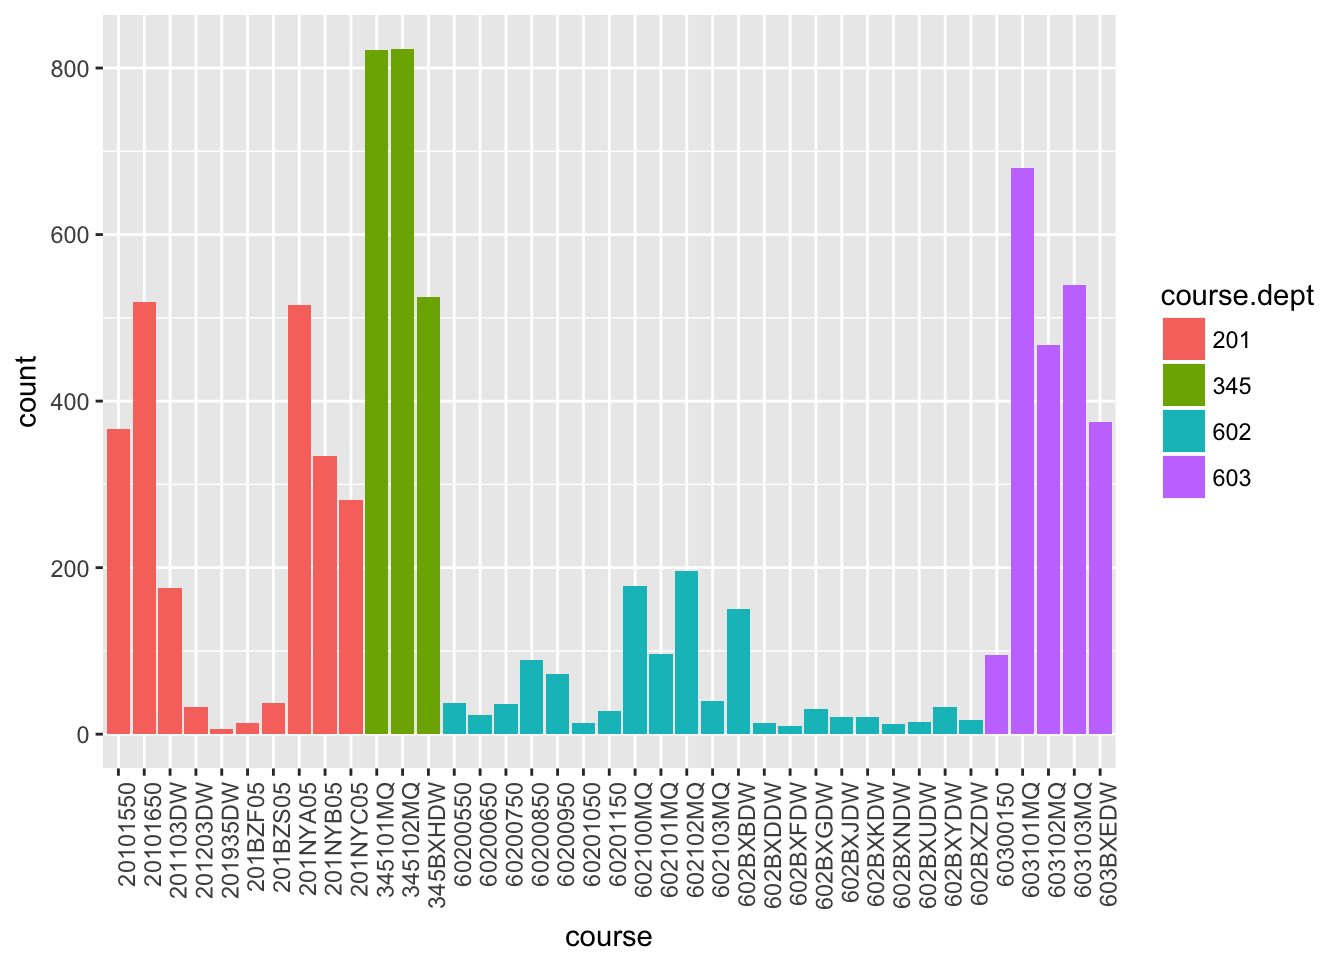
\includegraphics{studentsuccess_final_report_files/figure-latex/big-dept-seat-dist-by-course-1.pdf}

\subsection{Specialized spaces}\label{specialized-spaces}

If we look at the departments that require specialized spaces
(i.e.~labs), in 2016, how are the seats distributed by course? - Has
this evolved over time? - What are the seasonal variations?

\subsubsection{Winter}\label{winter}

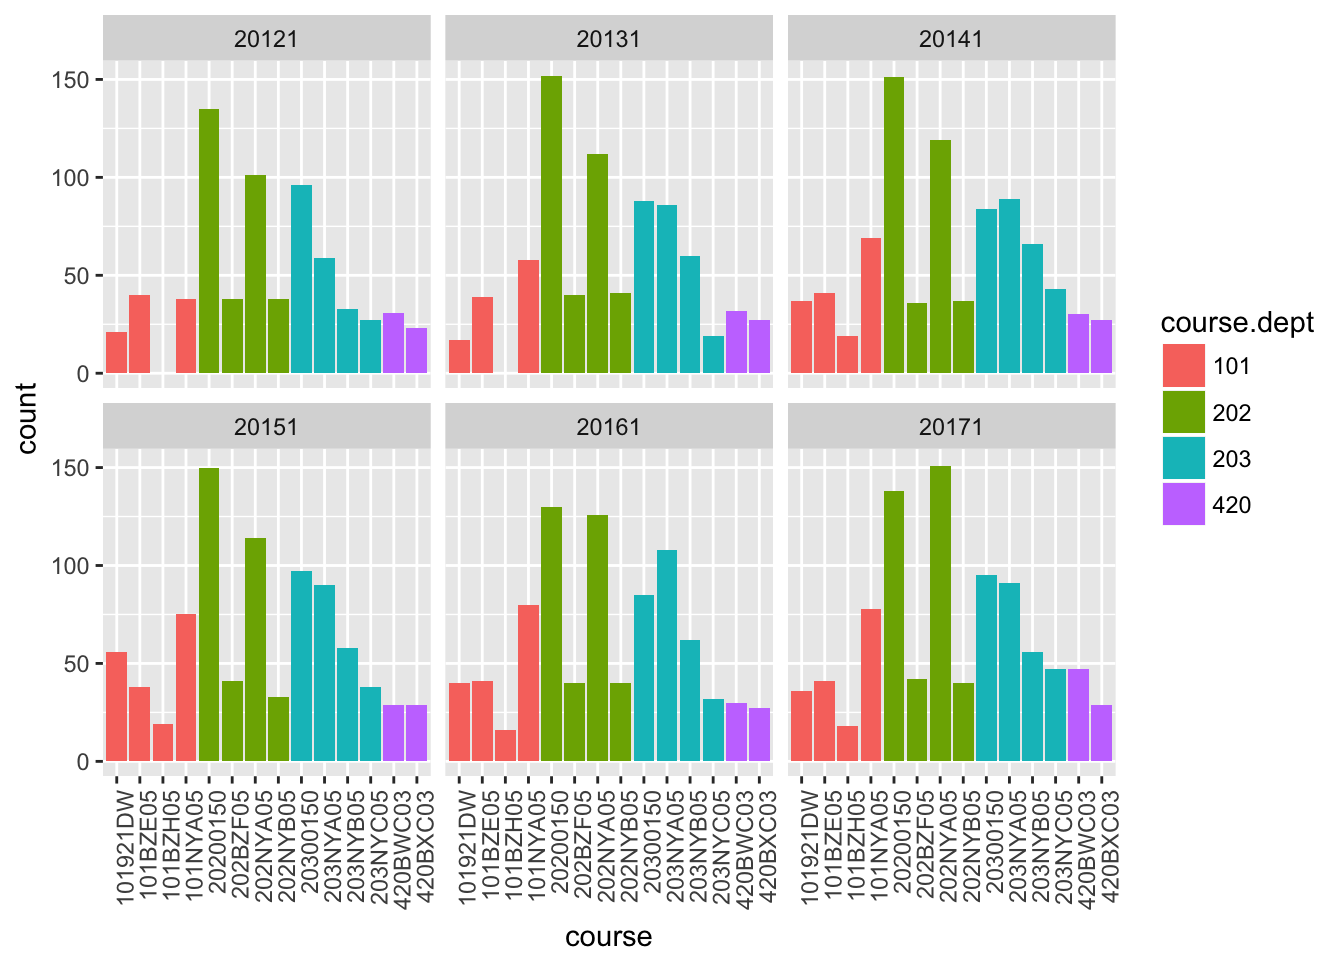
\includegraphics{studentsuccess_final_report_files/figure-latex/lab-dept-seat-dist-by-course-winter-1.pdf}

\subsubsection{Fall}\label{fall}

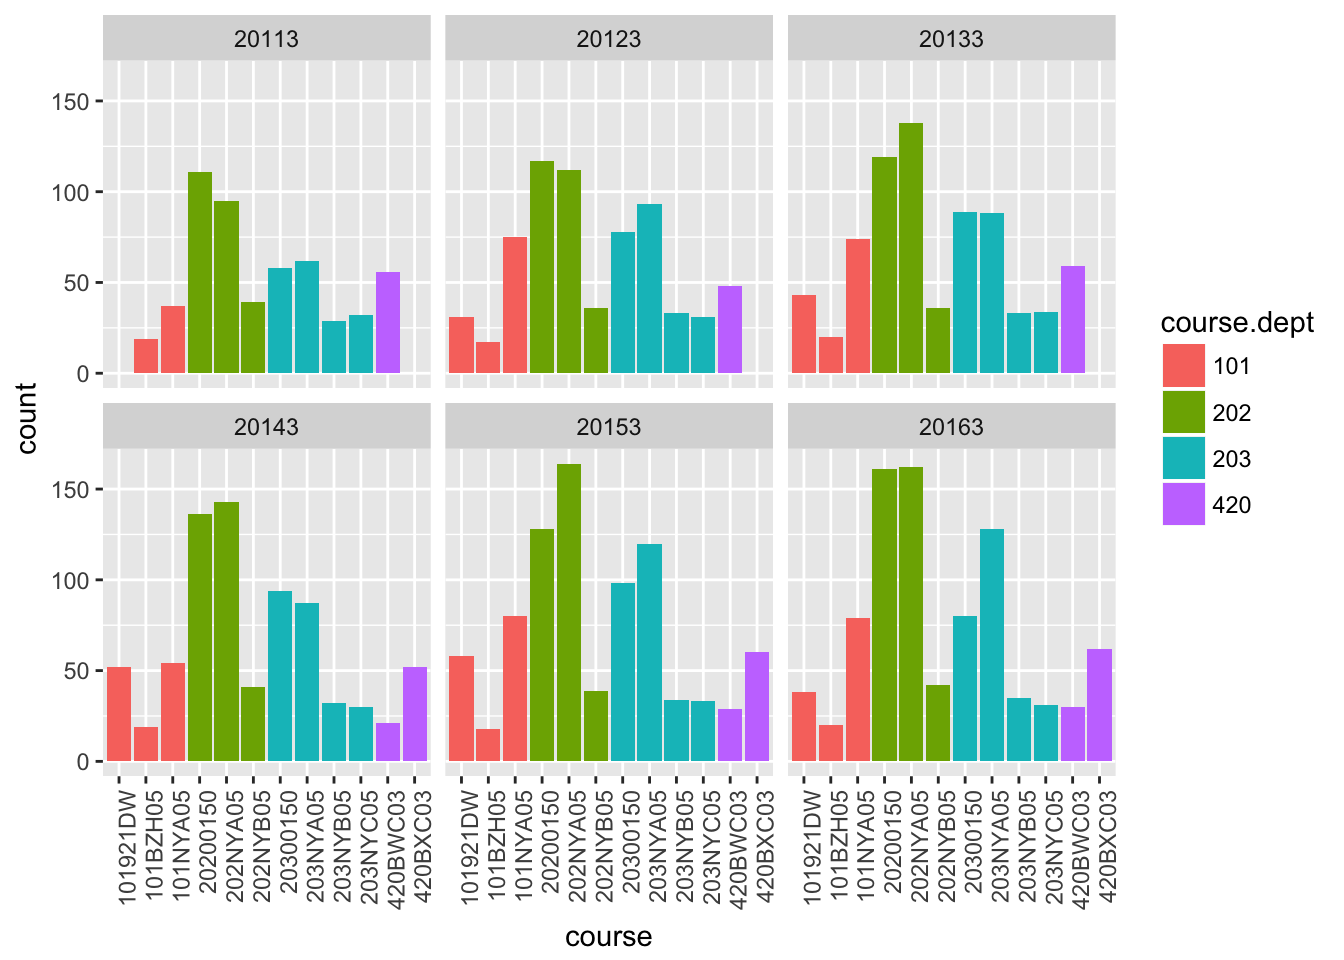
\includegraphics{studentsuccess_final_report_files/figure-latex/lab-dept-seat-dist-by-course-fall-1.pdf}

\subsubsection{Summer}\label{summer}

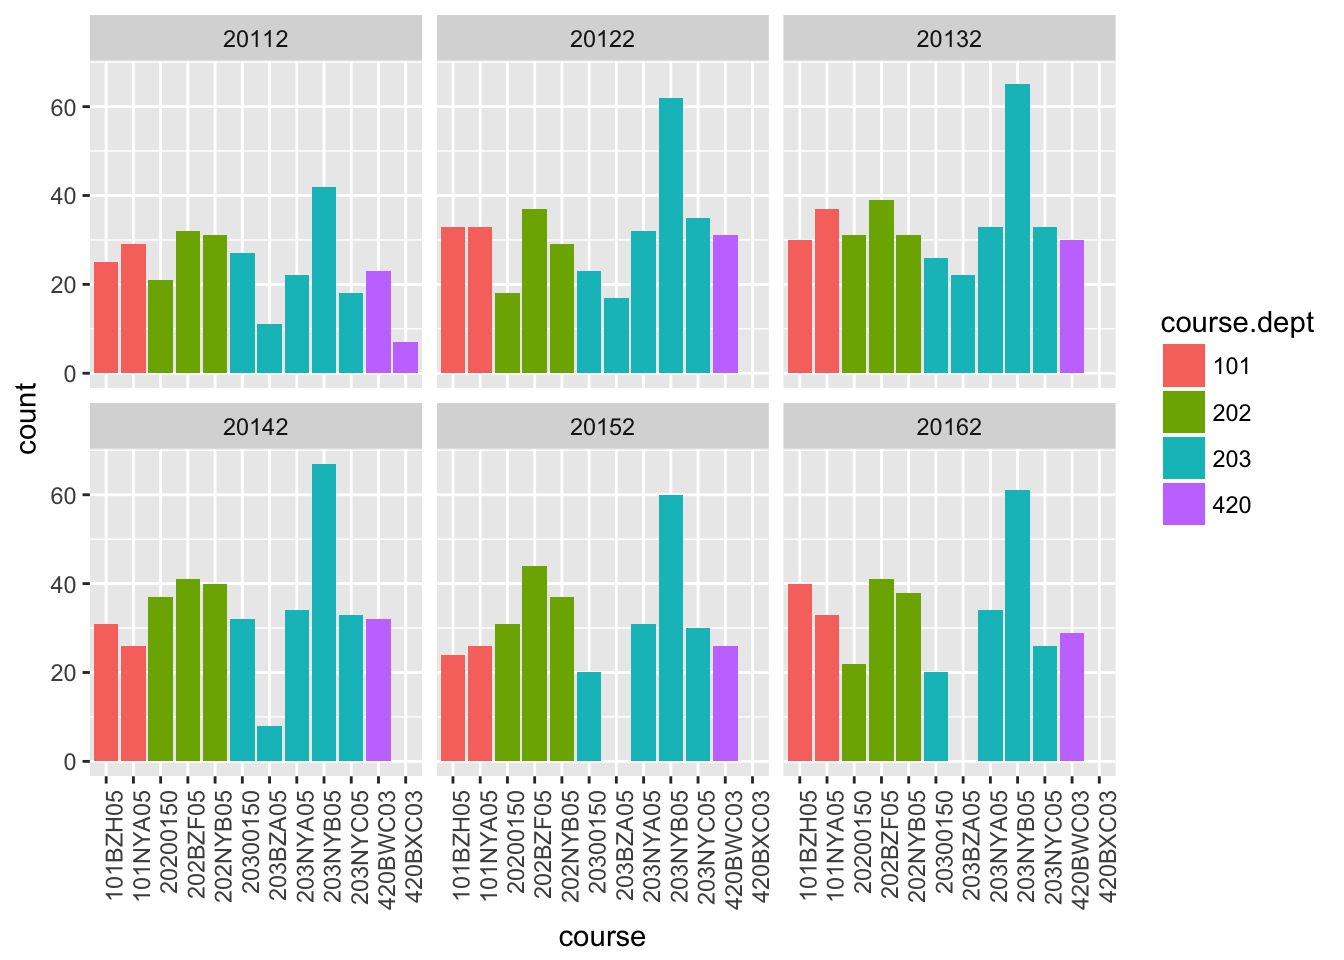
\includegraphics{studentsuccess_final_report_files/figure-latex/lab-dept-seat-dist-by-course-summer-1.pdf}

\section{Students}\label{students}

\subsection{Demographics}\label{demographics}

Who are the students using continuing education services?

\begin{itemize}
\tightlist
\item
  are there gender differences?
\item
  are there age differences?
\item
  do these demographics change over time?
\item
  are there seasonal variations?
\item
  are there differences in different departments?
\end{itemize}

\subsubsection{Sexe}\label{sexe}

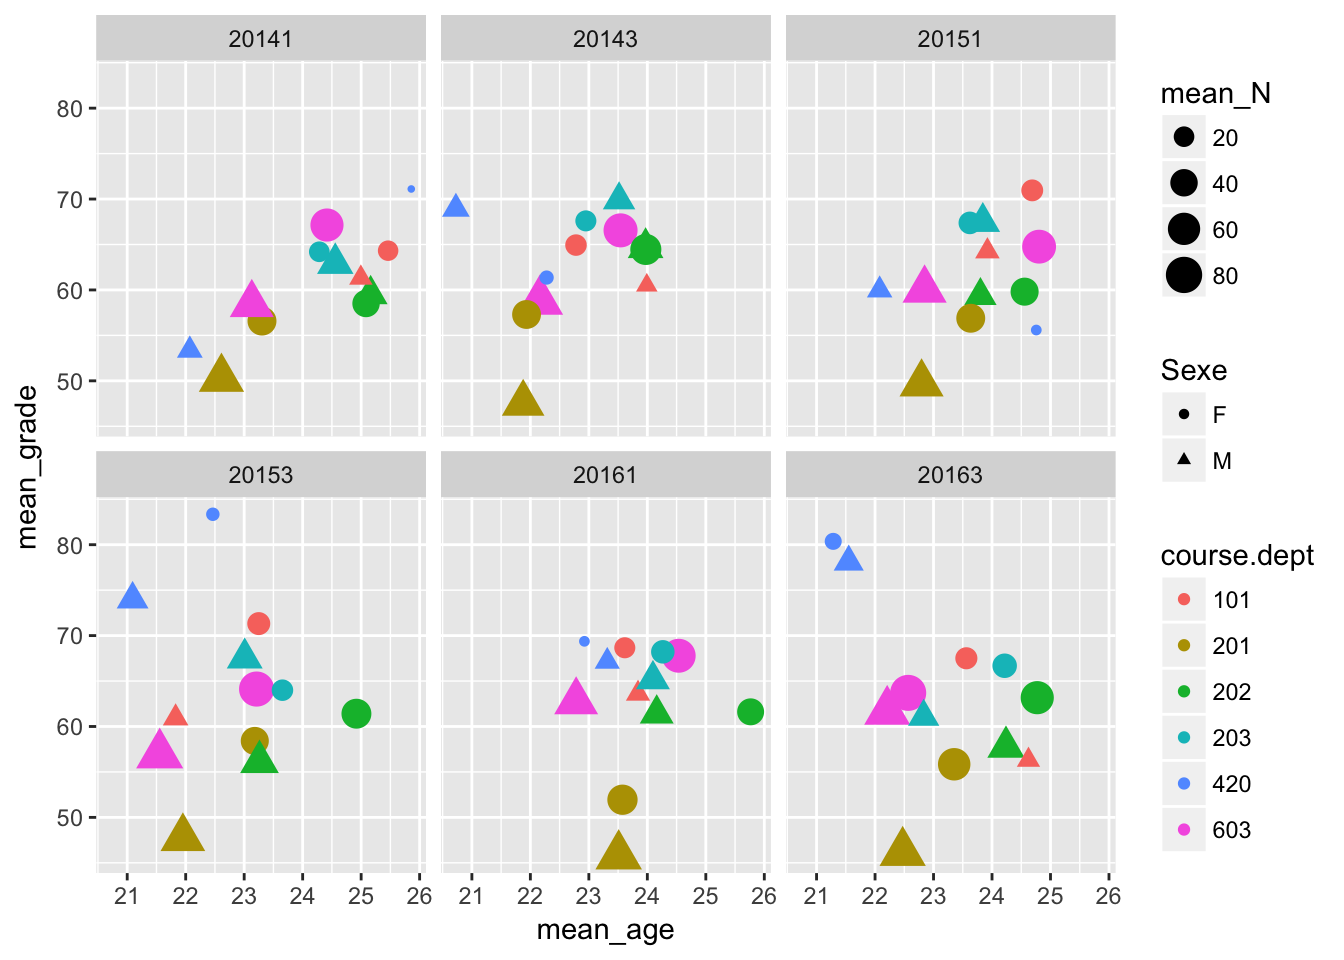
\includegraphics{studentsuccess_final_report_files/figure-latex/Sexe-demographics-over-time-1.pdf}

What is impact of condensed summer term?

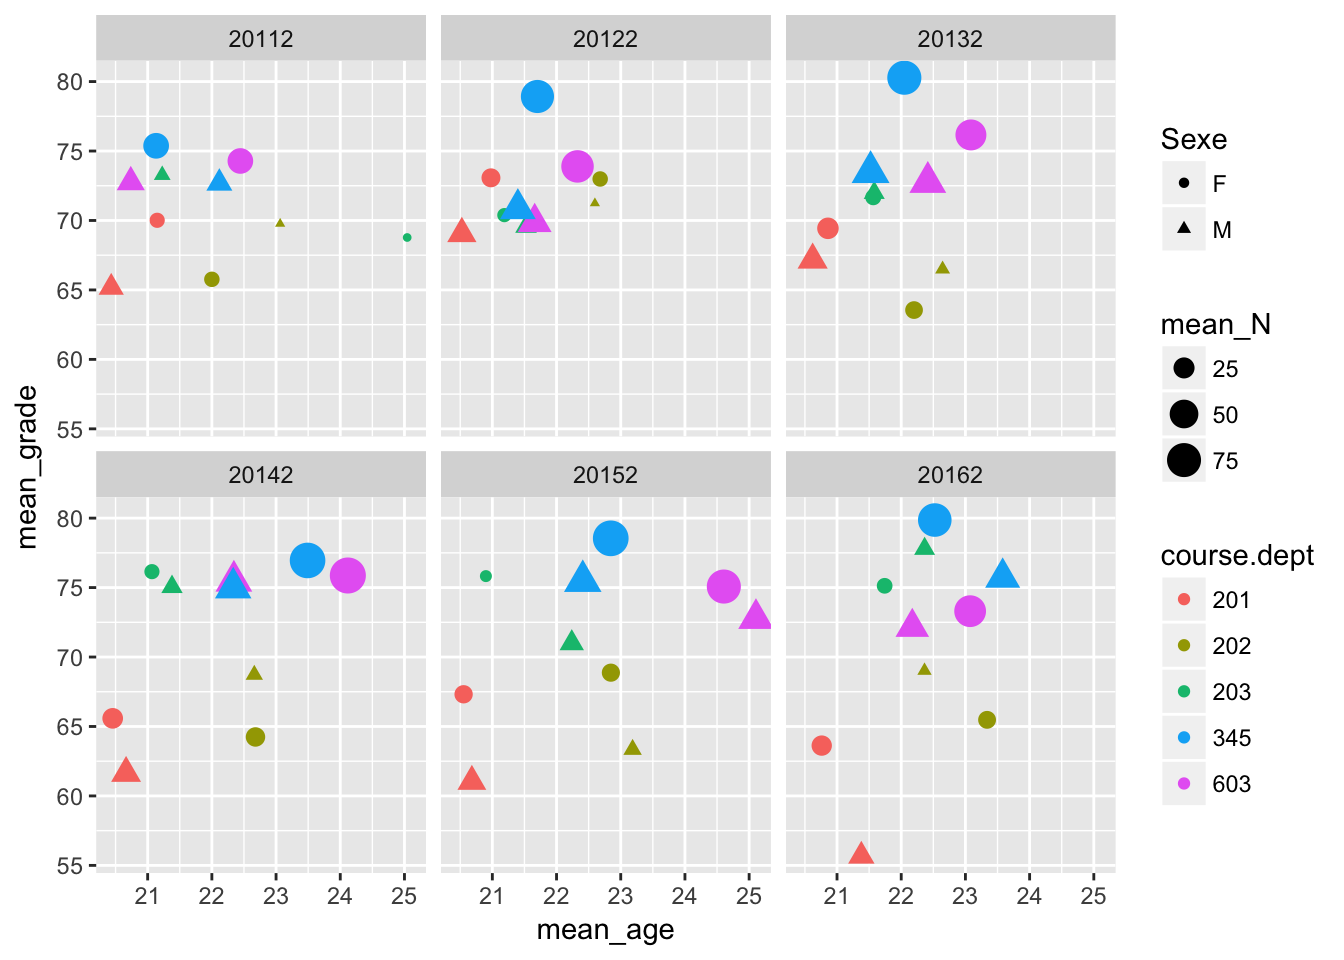
\includegraphics{studentsuccess_final_report_files/figure-latex/Sexe-demographics-over-time-summer-1.pdf}

\subsubsection{Birth Place}\label{birth-place}

Now, instead of looking at effect of gender, we focus instead on Birth
Place. To Quebec residents stand out in any consistent way, as compared
to those born elsewhere?

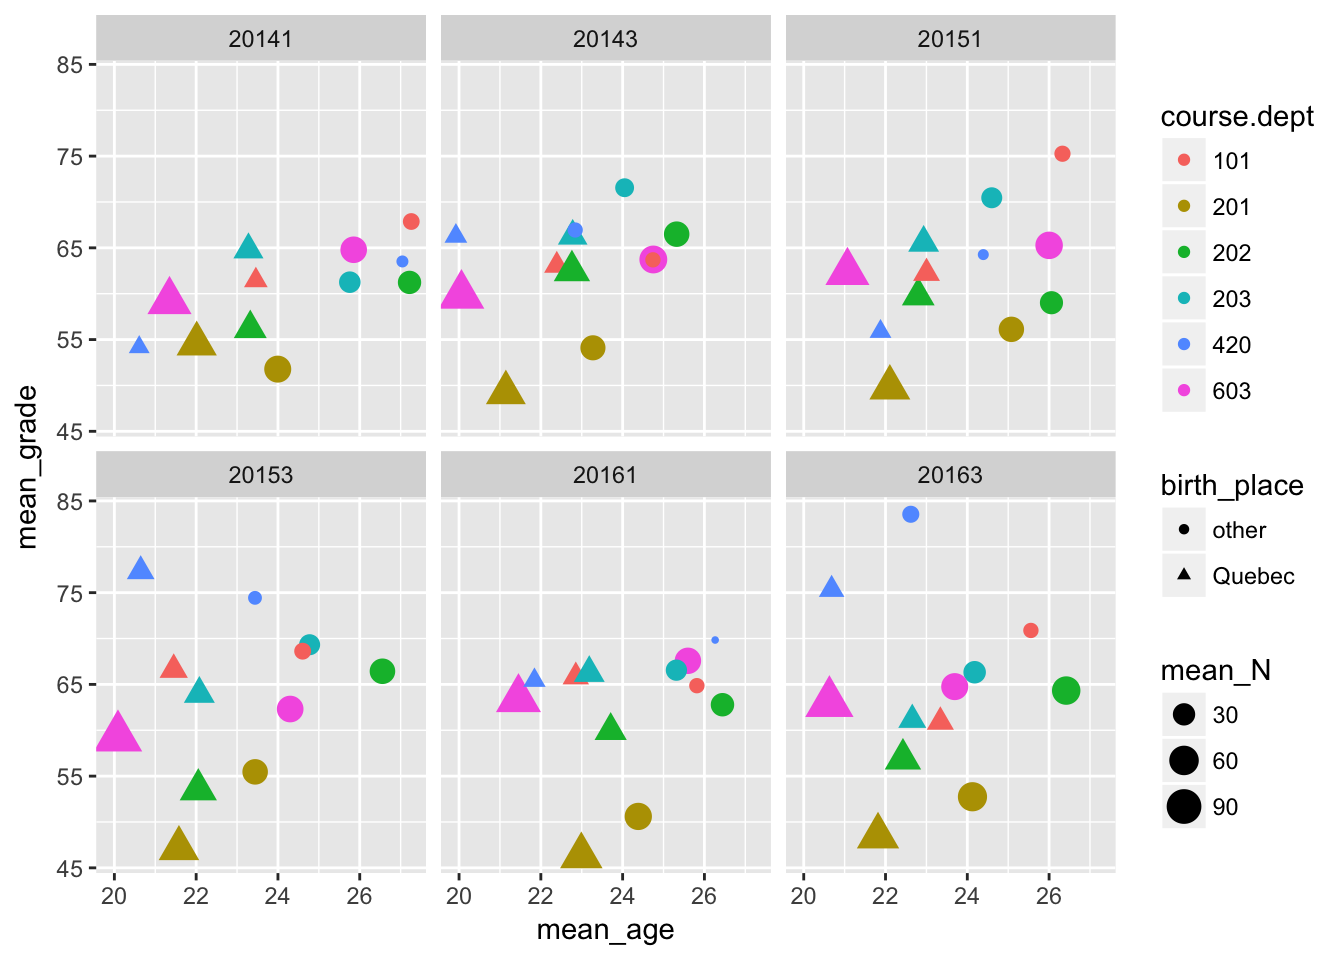
\includegraphics{studentsuccess_final_report_files/figure-latex/birth-place-demographics-over-time-1.pdf}

Again, what is impact of condensed summer term?

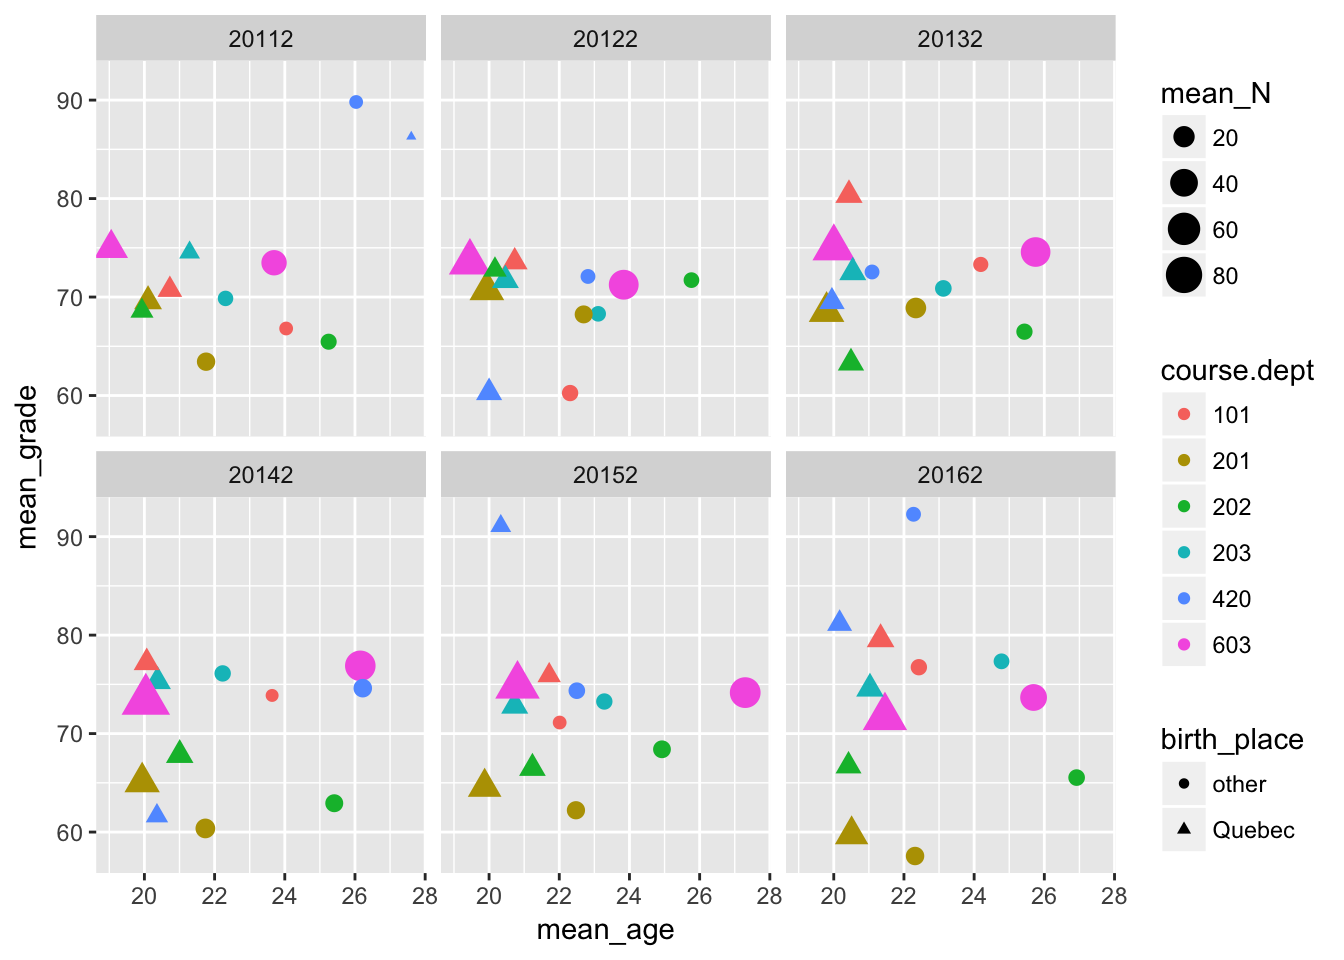
\includegraphics{studentsuccess_final_report_files/figure-latex/birth-place-demographics-over-time-summer-1.pdf}

\subsubsection{Mother Tongue}\label{mother-tongue}

Finally we look at the possible impact of Mother Tongue. How do
anglophones, francophones, and allophones compare in Continuing
Education?

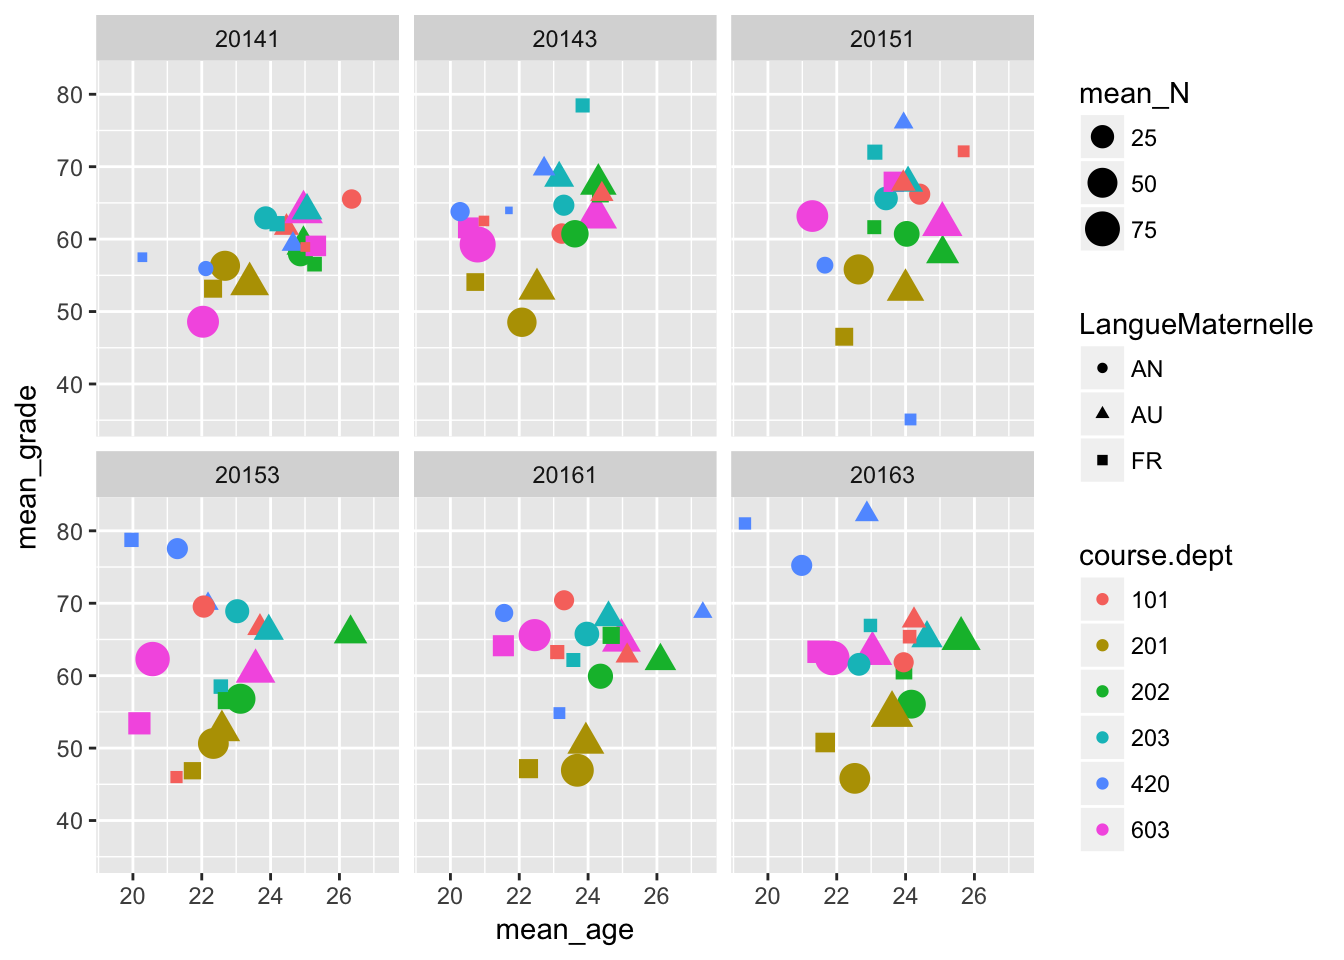
\includegraphics{studentsuccess_final_report_files/figure-latex/langue-demographics-over-time-1.pdf}

Again, what is impact of condensed summer term?

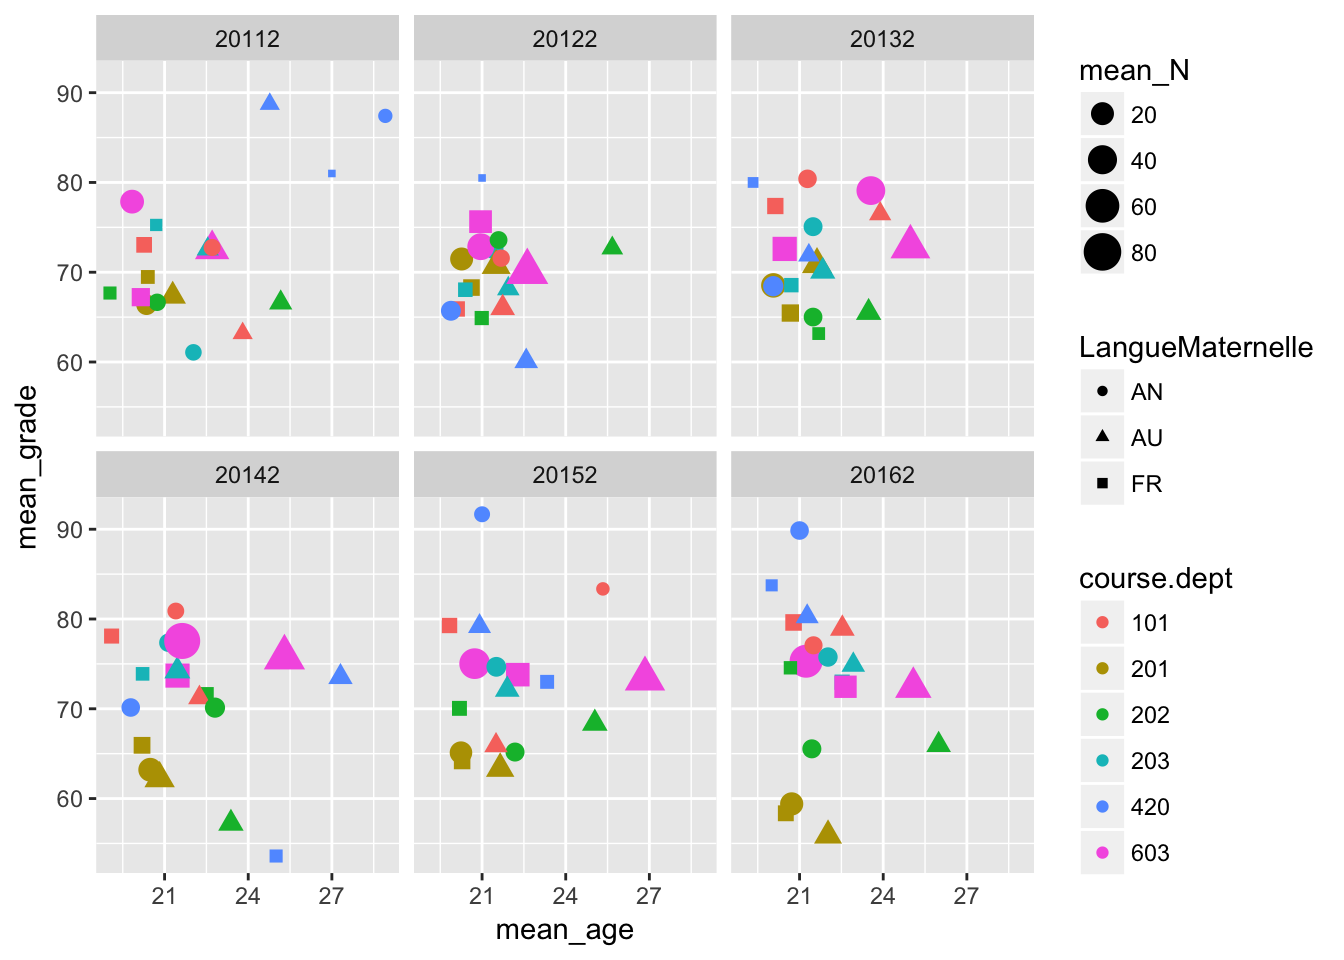
\includegraphics{studentsuccess_final_report_files/figure-latex/langue-demographics-over-time-summer-1.pdf}

\subsection{Success Rates}\label{success-rates}

To come\ldots{}

\chapter{Final Words}\label{final-words}

We have finished a nice book.

\bibliography{packages.bib,book.bib,studentsuccess.bib}


\end{document}
